\documentclass[a4paper,10pt]{article}
\usepackage[utf8]{inputenc}
\usepackage[spanish]{babel}
\usepackage{graphicx}
\usepackage{amssymb}

%opening
\title{\bf{Aprendizaje Automático Profundo\\ 
(Deep Learning)\\
Reporte Entregable 1}}
\author{Integrantes:\\
Candelaria Arpajou: mcarpajou@santafe-conicet.gov.ar\\
Hugo Folonier: hugofolonier@gmail.com\\
Gustavo Jaca: gustavojaca@gmail.com\\
Nicolas Rosales: elnicorosales@gmail.com}

\begin{document}

\maketitle

\begin{abstract}
Reporte correspondiente al primer entregable de la materia Aprendizaje Automático Profundo (Deep Learning). Presentamos los resultados de implementar una Red Neuronal Lineal Simple al problema Meli-Challenge-2019 con una pequeña exploracion de hiperparámetros. 
\end{abstract}

\section*{Modelo}

El modelo utilizado fué una Red Neuronal Lineal MLP:\\

$SuperSimpleMLP($

$  (embeddings): Embedding(50002, 300, padding_idx=0)
  (hidden_layer1): Linear(in_features=300, out_features=512, bias=True)
  (hidden_layer2): Linear(in_features=512, out_features=8192, bias=True)
  (hidden_layer3): Linear(in_features=8192, out_features=1024, bias=True)
  (output_layer): Linear(in_features=1024, out_features=632, bias=True)
)$\\

La función de Loss escogida fué $CrossEntropyLoss()$.\\

El optimizador escogido fué $SGD$, donde los hiperparámetros explorados fueron el learning rate $lr = (0.01, 0.05)$ y el momemtum $momemtum = (0.5, 0.9)$.\\

Para diferentes valores de hiperparámetros entrenamos la red con el conjunto de entrenamiento por 10 epocas. Al final de cada época guardamos la loss del conjunto de entrenamiento. Después evaluamos con el conjunto de validación y también guardamos la loss. Además guardamos el $balanced\_accuracy\_score$ de sklearn. Para completar, al final de las 10 epocas guardamor el $classification\_report$, también de sklearn.

\section*{Resultados}

Los resultados para la Loss, para los diferentes valores de los hiperparámetros pueden observarse en la Figura 1.

\begin{figure}[h]
\centering
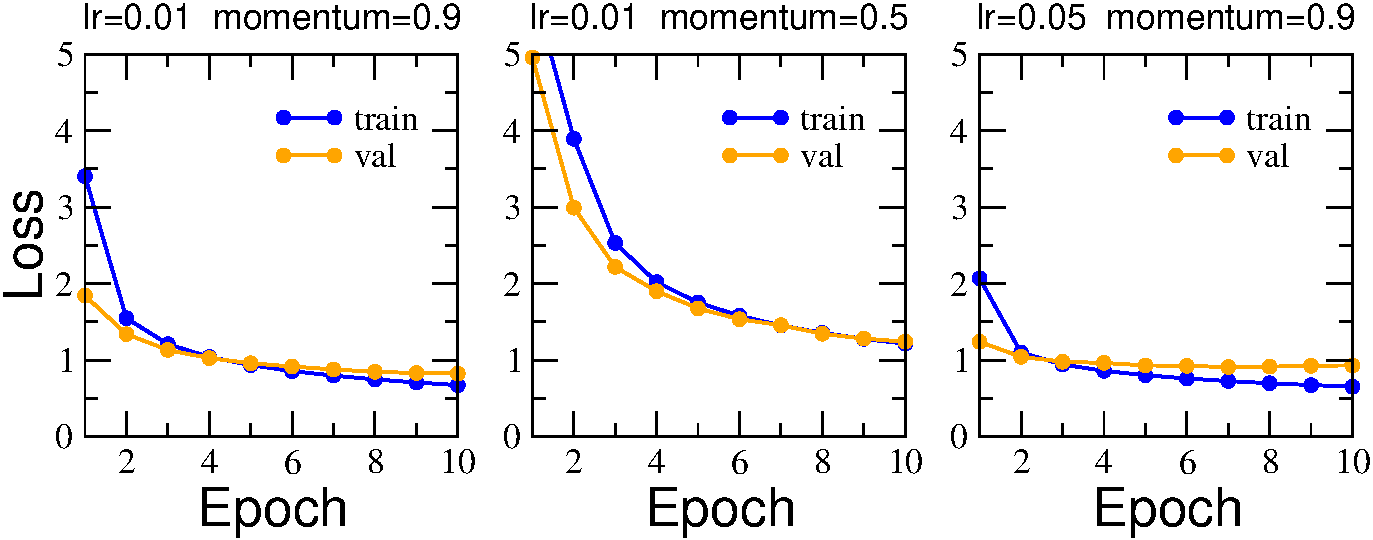
\includegraphics[scale=0.5]{data/loss-MLP.pdf}
\caption{Loss del dataframe train (azul) y del dataframe de validación (naranja) en funcion de las épocas para tres conjuntos de hiperparámetros $lr$ y $momentum$ diferentes.}
\label{fig01}
\end{figure}

Podemos observar que para $lr=0.05$ y $momentum=0.9$ (panel de la derecha, aka hip3), a pesar de que la loss del train continúa cayendo al cabo de 10 épocas, la loss de validación se estabiliza en torno de la épocas 3. Esto último significa que estaríamos en presencia de un sobreajuste. Para el conjunto de hiperparámetros $lr=0.01$ y $momentum=0.9$ (panel de la izquierda, aka hip1), a pesar de que ambas loss decaen al cabo de las 10 épocas de entrenamiento, parece que a partir de la época 7, la loss de validación empieza a decaer más lentamente que la loss del train. Finalmente, para el conjunto de hiperparámetros $lr=0.01$ y $momentum=0.5$ (panel del centro, aka hip2), al final de las 10 épocas iniciales, ámbas loss continúan cayendo y ámbas tienen valores muy altos, por lo que corresponde a un modelo más ineficiente que los anteriores. 

\begin{figure}[h]
\centering
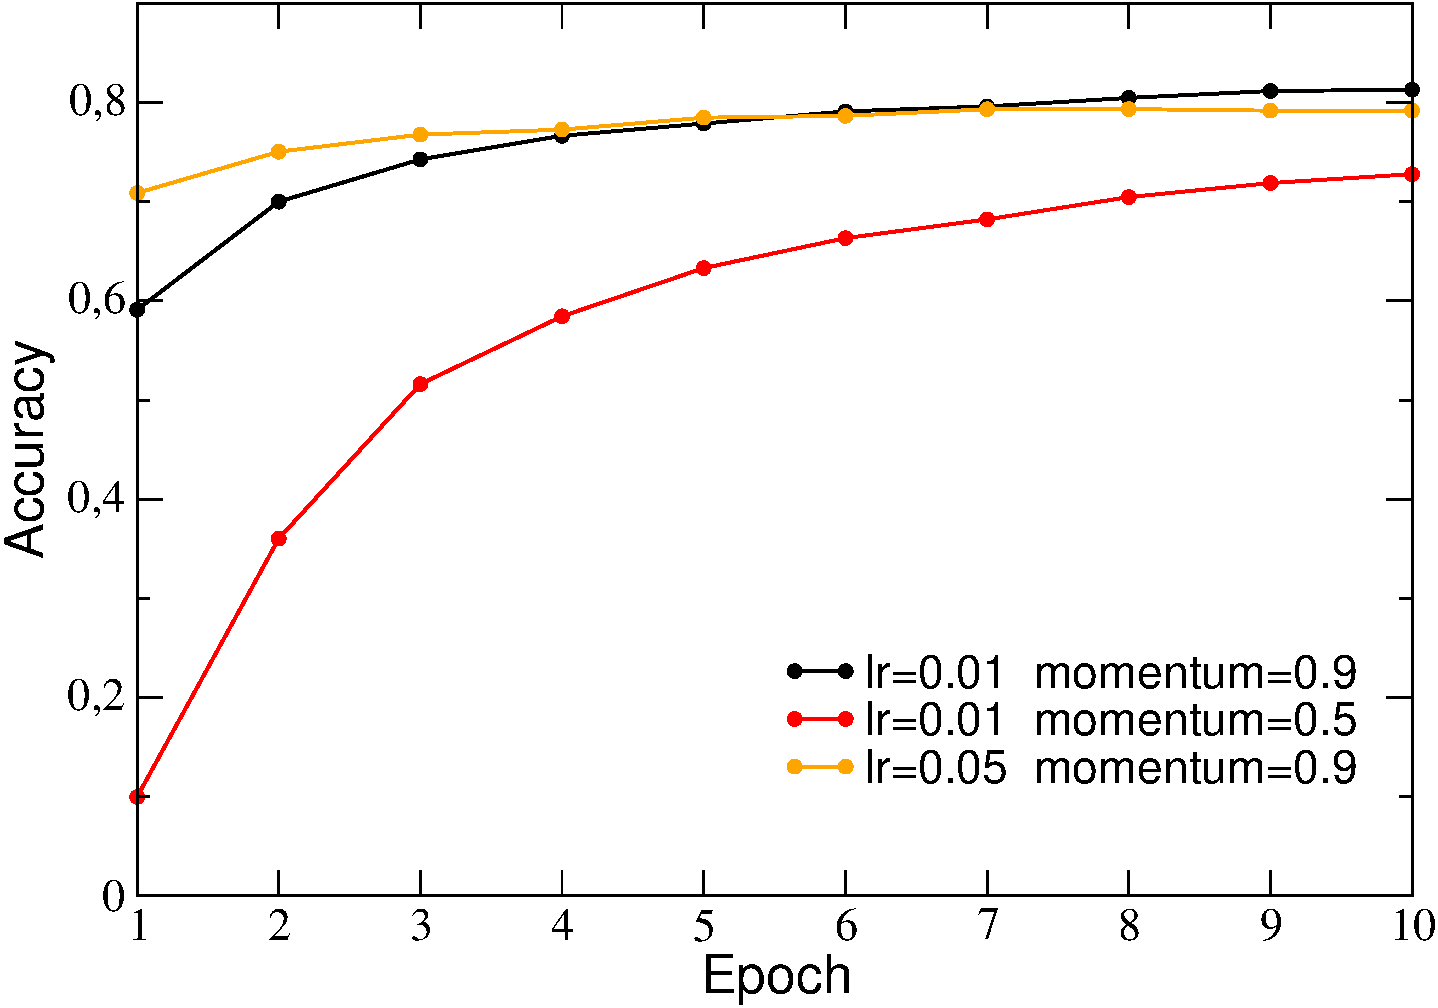
\includegraphics[scale=0.35]{data/accuracy-MLP.pdf}
\caption{Balanced accuracy score del dataframe de validación en funcion de las épocas para tres conjuntos de hiperparámetros $lr$ y $momentum$ diferentes.}
\label{fig02}
\end{figure}

En la Figura 2 graficamos métrica balanced accuracy score para el conjunto de validación al final de cada época de entrenamiento. En esta figura puede obervarse claramente que el conjunto hip2 (curva roja) es el menos preciso al cabo de 10 épocas. Para los conjuntos de hiperparámetros hip1 e hip3, ámbas curvas son bastante similares. Entre las épcocas 
1 y 5 el conjunto hip3 es más preciso, estabilizando su valor de accuracy a un valor casi constante, miemtras que entre las épcocas 5 y 10 el conjunto hip1 es más preciso. Esto es consistente con las curvas de loss de la Figura 1.

Finalmente, el Cuadro 1 resume el accuracy calculado con $classification\_report$ de sklearn, sobre el dataframe de test usando el modelo generado por cada conjunto de hiperparámetros al final de las 10 épocas de entrenamiento.
\begin{table}[h]
\caption{Accuracy final para los diferentes conjuntos de hiperparámetros.}\label{tab:data}
\begin{tabular}{cc}
\hline
Hiperparámetros  & accuracy \\
\hline
\hline
$lr=0.01; momentum=0.9$ &  0.87\\
$lr=0.01; momentum=0.5$ &  0.79\\
$lr=0.05; momentum=0.9$ &  0.85
\end{tabular}
\end{table}

Como futuros pasos a seguir promopenos una exloración más euxastiva de los hiperparámetros, y principalmente en el diseño de las capas lineales de la red. Una red más profunda (con más tiempo de entrenamiento), probablemente ayude a incrementar el accuracy sobre el contunto de testeo.

\end{document}
